\section{Node.js}

\begin{defi}{Node.js}
    \begin{wrapfigure}{r}{0.25\textwidth}
        \begin{center}
            
\includegraphics[width=0.2\textwidth]{includes/figures/defi_node_js.png}
        \end{center}
    \end{wrapfigure}

    Neben clientseitigem JavaScript kann man ebenfalls serverseitig dynamisch HTML-Objekte erstellen.
    Viele serverseitige Methoden nutzen die selbe Syntax wie clientseitige Methoden.

    Node.js ist ein eventbasierter Webserver.
    Bei einer Anfrage wird ein Thread erstellt, welcher genutzt wird, um diese synchron abzuarbeiten.
    Der Haupt Thread wird dabei jedoch nicht blockiert.
    Jeder Worker-Thread läuft dabei in einer eigenen JavaScript Engine.

    Ein erster Ansatz sieht wie folgt aus\footnote{Node.js erstellt einen Worker Thread (hier blau)}:
    \begin{center}
        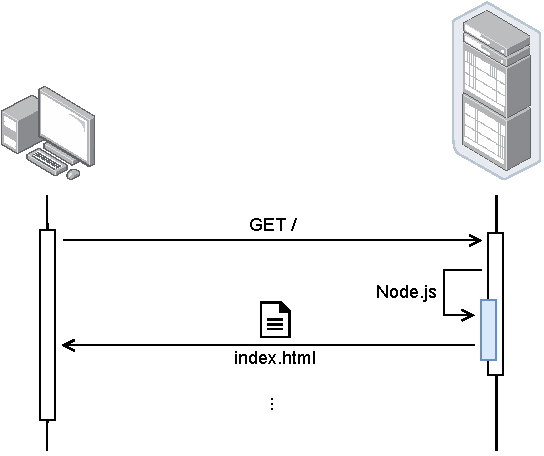
\includegraphics[width=0.5\textwidth]{includes/figures/defi_js_server.pdf}
    \end{center}
    Auf dem Server existiert potentiell keine Datei \texttt{index.html}, sondern wird immer neu erstellt.
\end{defi}

\begin{example}{Ordnerstruktur (Node.js)}
    \begin{center}
        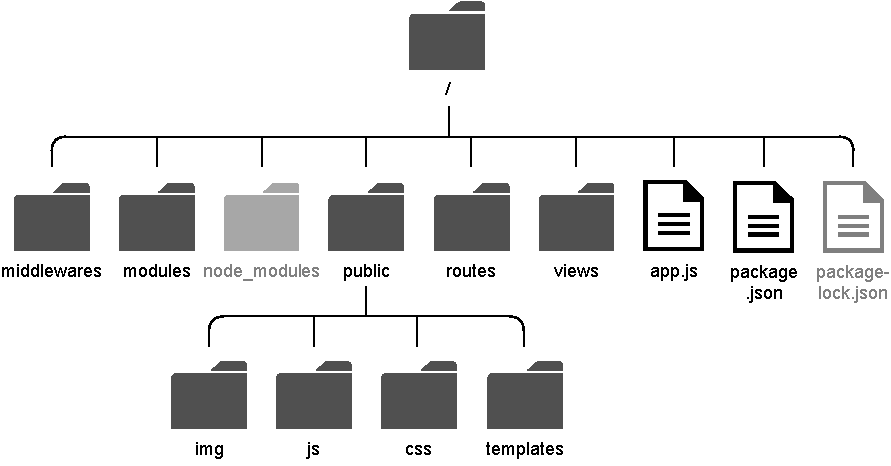
\includegraphics[width=0.75\textwidth]{includes/figures/example_nodejs_ordnerstruktur.pdf}
    \end{center}
\end{example}

\subsection{package.json}

\begin{bonus}{package.json (Node.js)}
    \begin{center}
        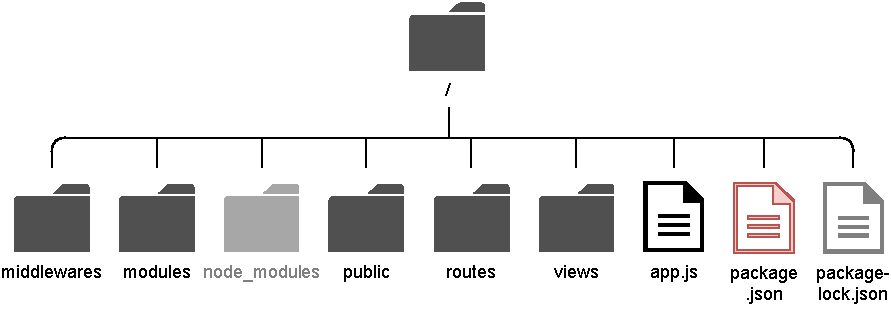
\includegraphics[width=0.75\textwidth]{includes/figures/bonus_nodejs_package.pdf}
    \end{center}

    \texttt{npm init} erzeugt interaktiv eine \texttt{package.json}, welche Informationen über das Node Projekt (wie z. B. Abhängigkeiten) enthält.
    Enthält der Ordner diese \texttt{package.json} wird sie von Node als Projekt erkannt und kann mit \texttt{node .} ausgeführt werden.
\end{bonus}

\begin{defi}{Module}
    Ein Module ist eine Funktionalität, die in eine eigene JavaScript Datei ausgelagert wurde.

    Man unterteilt JavaScript Module in drei Arten:
    \begin{enumerate}
        \item Integrierte Module
              \begin{itemize}
                  \item Vorinstallierte Kernmodule
              \end{itemize}
        \item Lokale Module
              \begin{itemize}
                  \item Meist selbstgeschriebene Funktionen und Klassen
                  \item Zu finden in \texttt{/modules}
              \end{itemize}
        \item Third Party Module
              \begin{itemize}
                  \item Öffentliche Module, welche per Package Manager eingebunden werden müssen
                  \item Zu finden in \texttt{/node\_modules}
              \end{itemize}
    \end{enumerate}

    Zum Nutzen der Module muss man ganz oben in seine JavaScript-Datei folgende import-Anweisung nutzen:
    \begin{lstlisting}[language=JavaScript]
        const MODULE = require('/modules/file.js')
    \end{lstlisting}
\end{defi}

\subsection{modules}

\begin{bonus}{modules (Node.js)}
    \begin{center}
        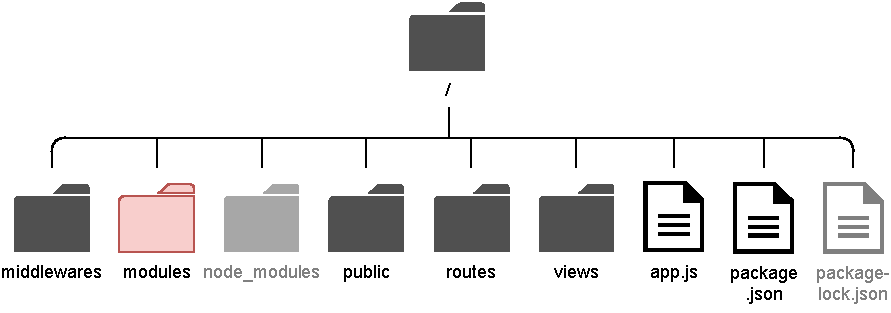
\includegraphics[width=0.75\textwidth]{includes/figures/bonus_nodejs_module.pdf}
    \end{center}

    Zum Exportieren seiner Funktion muss man nach der Initialisierung der Methode bzw. Klasse folgendes export-Anweisung nutzen:
    \begin{lstlisting}[language=JavaScript]
        module.exports = ...
    \end{lstlisting}
\end{bonus}

\begin{example}{modules (Node.js)}
    Um Klassen direkt zu exportieren, kann man \texttt{module.exports} überschreiben.

    \texttt{modules/pokemon.js}
    \begin{lstlisting}[language=JavaScript]
        ^class Pokemon^ {
            id, name

            constructor(id, name) {
                this.id = id,
                this.name = name
            }

            to_string() {
                return `${this.name} [${this.id}]`
            }
        }

        module.exports = Pokemon
    \end{lstlisting}

    \texttt{app.js}
    \begin{lstlisting}[language=JavaScript]
        const ^Pokemon^ = require('./modules/pokemon.js')

        const glumanda = ^new Pokemon(4, 'Glumanda')^
        console.log(glumanda.to_string()) // Glumanda [4]
    \end{lstlisting}
\end{example}

\begin{example}{modules (Node.js)}
    Alternativ kann man direkt Instanzen exportieren (z. B. für Singleton etc.):

    \texttt{modules/pokemon.js}
    \begin{lstlisting}[language=JavaScript]
        class Pokemon { ... }

        module.exports = ^new Pokemon(4, 'Glumanda')^
    \end{lstlisting}

    \texttt{app.js}
    \begin{lstlisting}[language=JavaScript]
        const ^glumanda^ = require('./modules/pokemon.js')

        console.log(glumanda.to_string()) // Glumanda [4]
    \end{lstlisting}
\end{example}

\begin{example}{modules (Node.js)}
    Um mehrere Objekte zu exportieren, kann man entweder \texttt{module.exports}\footnote{
        Wenn man nur das Objekt anpasst, kann man \texttt{exports = ...} nutzen, da \texttt{exports} ein pointer auf \texttt{module.exports} ist.
        Beim Überschreiben der Variable wird nur die Referenz auf \texttt{module.exports} gelöscht.
    } anpassen oder mit einem Array überschreiben.

    \texttt{modules/pokemon.js} (exports)
    \begin{lstlisting}[language=JavaScript]
        class Pokemon { ... }
        class Attacke { ... }
        function brennen(p) { ... }

        /* module. */ exports.Pokemon = Pokemon
        /* module. */ exports.Attacke = Attacke
        /* module. */ exports.brennen = brennen
    \end{lstlisting}

    \texttt{app.js}
    \begin{lstlisting}[language=JavaScript]
        const pokemon_module = require('./modules/pokemon.js')

        pokemon_module.brennen(new pokemon_module.Pokemon(4, 'Glumanda'))
    \end{lstlisting}

    oder:

    \texttt{modules/pokemon.js} (Array)
    \begin{lstlisting}[language=JavaScript]
        class Pokemon { ... }
        class Attacke { ... }
        function brennen(p) { ... }

        module.exports = [Pokemon, Attacke, brennen]
    \end{lstlisting}

    \texttt{app.js}
    \begin{lstlisting}[language=JavaScript]
        const [Pokemon, Attacke, brennen] = require('./modules/pokemon.js')

        brennen(new Pokemon(4, 'Glumanda'))
    \end{lstlisting}

    Man sieht, dass man in der ersten Variante deutlich mehr schreiben muss, da man den \enquote{namespace} vor jedes Objekt des Modules schreiben muss.
    Jedoch hat sie den deutlichen Vorteil, dass man nicht alle imports anpassen muss, wenn man einen export hinzufügt.
\end{example}

\subsection{node\_modules}

\begin{defi}{Node Package Manager}
    Node Package Manager (npm) ist ein Projektmanager für Node.js.
    Er wird genutzt um Öffentliche Module zu importieren oder eigene Module öffentlich zur Verfügung zu stellen.
\end{defi}

\begin{bonus}{node\_modules (Node.js)}
    \begin{center}
        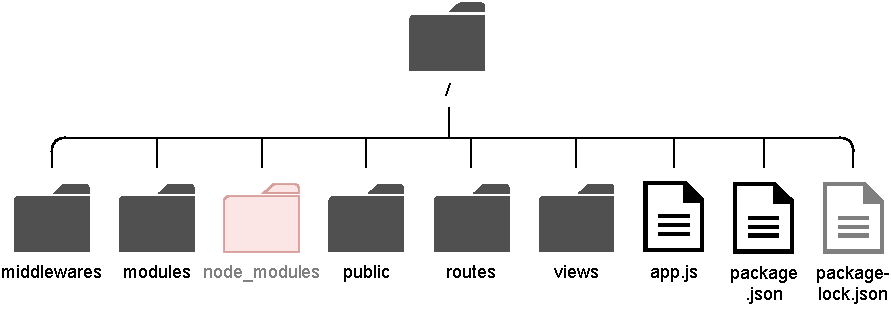
\includegraphics[width=0.75\textwidth]{includes/figures/bonus_nodejs_node_modules.pdf}
    \end{center}

    Um ein öffentliches Modul seiner \texttt{package.json} hinzuzufügen und dieses direkt zu laden, nutzt man:
    \texttt{npm install <package>}

    Wenn eine fremde \texttt{package.json} eingebunden hat und alle Module laden möchte, von denen das Projekt abhängig ist, nutzt man:
    \texttt{npm install}
\end{bonus}

\subsection{app.js}

\begin{bonus}{app.js (Node.js)}
    \begin{center}
        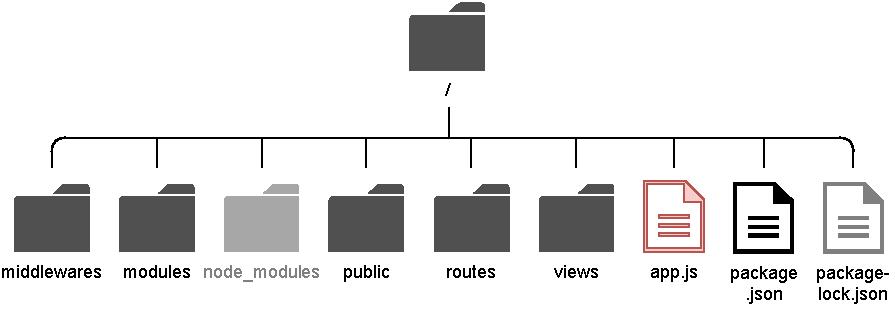
\includegraphics[width=0.75\textwidth]{includes/figures/bonus_nodejs_app.pdf}
    \end{center}

    Die \texttt{app.js} ist der Einstiegspunkt für unseren Server.
    In der \texttt{package.json} wird festgelegt, welche Datei diese Aufgabe übernimmt.

    Der Server wird mit \texttt{node .} gestartet.
\end{bonus}

\begin{example}{app.js (Node.js)}
    Ein reiner Webserver kann wie folgt erstellt werden.
    Es wird ausschließlich das vorinstallierte Modul \emph{http} benötigt.

    \begin{lstlisting}[language=JavaScript]
        const http = require('http')

        const port = 3000

        function handleRequest(req, res) {
            res.end(req.url + ': hello')
        }

        const server = http.createServer(handleRequest)
        server.listen(port)
    \end{lstlisting}

    Wenn man nun z. B. die Webseite \texttt{http://localhost:3000/test} aufruft, erhält man:\\
    \texttt{/test: hello}
\end{example}

\begin{defi}{express (Node.js)}
    \emph{express} ist das meistgenutzte Web-Framework für Node.js.
    Es erweitert Node.js um Werkzeuge, mit denen das Entwickeln moderner Webanwendungen einfacher gestaltet wird
\end{defi}

\begin{example}{app.js (Node.js)}
    \begin{lstlisting}[language=JavaScript]
        const express = require('express')
        
        const app = express()
        const port = 3000

        app.get('/', (req, res) => {
            res.send('hello')
        })

        app.listen(port)
    \end{lstlisting}

    Wenn man nun die Webseite \texttt{http://localhost:3000/} aufruft, erhält man:\\
    \texttt{hello}

    Die Routen werden jedoch meist nicht in der \texttt{app.js} definiert, sondern lediglich eingebunden:
    \begin{lstlisting}[language=JavaScript]
        app.use(require('routes/file.js'))
    \end{lstlisting}
\end{example}

\subsection{routes}

\begin{bonus}{routes (Node.js)}
    \begin{center}
        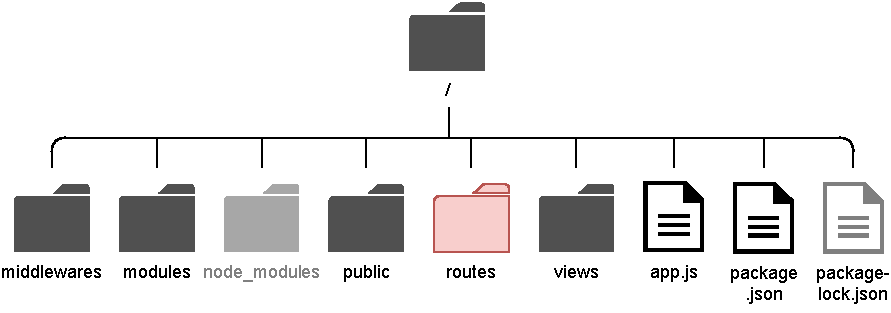
\includegraphics[width=0.75\textwidth]{includes/figures/bonus_nodejs_routes.pdf}
    \end{center}
\end{bonus}

\begin{defi}{Route}
    Routen dienen zur Navigation innerhalb einer Anwendung.

    Sie werden als Callback-Methode abgebildet:
    \texttt{.get('/'. (req, res, next) => {})}

    Die Syntax besteht aus folgenden Teilen:
    \begin{itemize}
        \item \emph{HTTP Methode}: z. B. \texttt{get}, \texttt{post}, \texttt{put}, \texttt{patch}, \texttt{delete} etc.
              Alternativ:
              \begin{itemize}
                  \item \texttt{all}: Alle \emph{HTTP Methoden}
                  \item \texttt{use}: Alle \emph{HTTP Methoden} inkl. rekursiv aller sub-Routen
              \end{itemize}
        \item \emph{Path}: Route, die im Browser genutzt wird. z. B. '/'

              Mögliche Eingaben: \texttt{string}, \texttt{muster}, \texttt{regulärer Ausdruck}, \texttt{array}
        \item \texttt{req}: \emph{HTTP request argument} mit übergebenen Parametern
        \item \texttt{res}: \emph{HTTP response argument}, welches wir hier erstellen

              \emph{Responses} sind z. B.:
              \begin{itemize}
                  \item \texttt{res.download()}: Fordert den Client auf, eine Datei herunterzuladen
                  \item \texttt{res.end()}: Beendet den Prozess
                  \item \texttt{res.json()}: Sendet ein JSON-Objekt
                  \item \texttt{res.jsonp()}: Sendet ein JSONP-Objekt
                  \item \texttt{res.redirect()}: Leitet den Client weiter
                  \item \texttt{res.render()}: Rendert eine Anzeigevorlage
                  \item \texttt{res.send()}: Sendet eine Antwort mit beliebigem Typen
                  \item \texttt{res.sendFile()}: Sendet eine Datei als Oktett-Stream
                  \item \texttt{res.sendStatus()}: Legt den Antwortstatuscode fest
              \end{itemize}
        \item \texttt{next}: Callback-Methode die ausgeführt werden muss, sollten wir weitere Routen haben, die unter dem Pfad liegen.
              Wenn \texttt{next()} genutzt wird, befinden wir uns in einer Middleware
    \end{itemize}
\end{defi}

\begin{defi}{Router}
    Wenn man mehrere Routen bündeln möchte, nutzt man Router.
    Man schafft eine Hierarchie um Sub-Pfade getrennt von den Routern zur Verfügung zu stellen und die Routennamen, falls nötig, zu parametrisieren.

    Eine Ansammlung von Routern findet man in \texttt{/routes}
\end{defi}

\begin{example}{Router}
    \begin{lstlisting}[language=JavaScript]
        app.get(^'/base_route/a'^, (req, res) => { ... })
        app.get(^'/base_route/b'^, (req, res) => { ... })
        app.get(^'/base_route/c'^, (req, res) => { ... })
    \end{lstlisting}

    wird vereinfacht zu:

    \begin{lstlisting}[language=JavaScript]
        const router = express.Router()

        router.get('/a', (req, res) => { ... })
        router.get('/b', (req, res) => { ... })
        router.get('/c', (req, res) => { ... })

        app.use(^'base_route'^, router)
    \end{lstlisting}
\end{example}

\begin{example}{routes (Node.js)}
    \texttt{app.js}:
    \begin{lstlisting}[language=JavaScript]
        const express = require('express')
        const app = express()

        /* routes */
        app.use(^'/pokemon'^, require('./modules/pokemon.js'))

        app.listen(3000)
    \end{lstlisting}

    \texttt{routes/pokemon.js}:
    \begin{lstlisting}[language=JavaScript]
        const Pokemon = require('./../modules/pokemon.js')
        const express = require('express')
        
        module.exports = express.Router()
            .get(^'/'^, (req, res) => {
                res.send(Pokemon.get_rand().to_string())
            })
            .get(^'/count'^, (req, res) => {
                res.send('896')
            })
    \end{lstlisting}

    Wenn man nun die Webseite \texttt{http://localhost:3000/pokemon} aufruft, erhält man z. B.:\\
    \texttt{Glumanda [4]}

    Wenn man die Webseite \texttt{http://localhost:3000/pokemon/count} aufruft, erhält man:\\
    \texttt{896}
\end{example}

\subsection{middlewares}

\begin{bonus}{middlewares (Node.js)}
    \begin{center}
        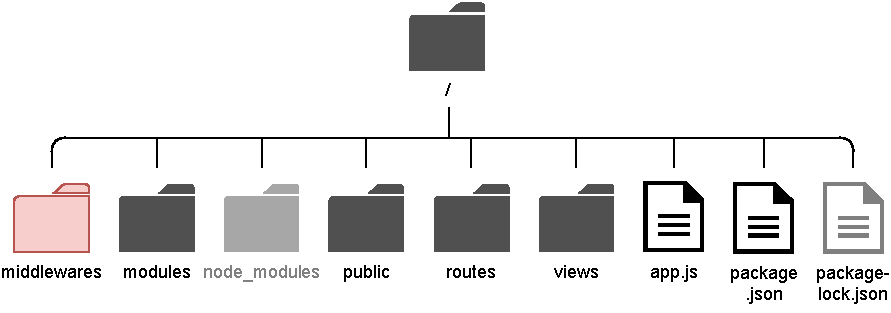
\includegraphics[width=0.75\textwidth]{includes/figures/bonus_nodejs_middlewares.pdf}
    \end{center}
\end{bonus}

\begin{defi}{Middleware}
    Middlewares sind ein Stack von Funktionen mit beliebigem Inhalt.
    Sie werden zwischen dem Eingehen eines Requests un dessen Bearbeitung durch einen Handler (z. B. Route) geschaltet.

    Sie haben Zugriff auf \emph{Request}, \emph{Response}, sowie die direkt folgende \emph{Middleware}.

    In Middlewares können z. B. Eingaben geparsed werden, geloggt werden oder Fehler abgefangen werden.
    Anmeldungen werden ebenfalls über Middlewares geregelt.
\end{defi}

\begin{example}{middlewares (Node.js)}
    \texttt{app.js}:
    \begin{lstlisting}[language=JavaScript]
        const express = require('express')
        const app = express()

        /* middlewares */
        app.use(^'/'^, require('./middlewares/logging.js')) // 1.
        
        /* routes */
        app.use(^'/pokemon'^, require('./modules/pokemon.js')) // 2.

        app.listen(3000)
    \end{lstlisting}

    \texttt{modules/pokemon.js}:
    \begin{lstlisting}[language=JavaScript]
        const Pokemon = require('./../modules/pokemon.js')
        const express = require('express')
        
        module.exports = express.Router()
            .get(^'/'^, (req, res) => {
                res.send(Pokemon.get_rand().to_string())
            })
    \end{lstlisting}

    \texttt{middlewares/logging.js}:
    \begin{lstlisting}[language=JavaScript]
        const express = require('express')
        
        module.exports = express.Router()
            .get(^'/*'^, (req, res, next()) => {
                console.log(req.url)
                ^next()^ // wichtig, da die Anfrage sonst hier abbricht
            })
    \end{lstlisting}

    Wenn man nun die Webseite \texttt{http://localhost:3000/pokemon} aufruft:
    \begin{enumerate}
        \item wird geloggt: \texttt{/pokemon}
        \item wird erhält man z. B.: \texttt{Glumanda [4]}
    \end{enumerate}
\end{example}

\subsubsection{Cookies}

\begin{defi}{Cookie}
    Der Zustand eines Node.js-Skriptes geht nach der Ausführung verloren.
    Clients wollen nicht immer alle Daten im Aufruf aktiv mitsenden und der Server möchte auch keine Daten zwischenspeichern.

    Deswegen lässt der Server Daten auf dem Client zwischenspeichern, die der Server nochmal benötigen könnte, damit der Client sie nicht nochmal aktiv senden muss.

    Cookies werden z. B. genutzt damit sich der Client einmalig anmelden kann, und dann angemeldet bleibt oder um das Nutzungsverhalten zu analysieren.

    Die Syntax um Cookies zu erstellen sieht wie folgt aus:
    \begin{lstlisting}[language=JavaScript]
        res.cookie('<name>', '<value>', options)
    \end{lstlisting}

    \begin{itemize}
        \item \texttt{name}: key des cookies
        \item \texttt{value}: value
        \item \texttt{options}: z. B.: \texttt{expires}, \texttt{path}, \texttt{domain} etc.
    \end{itemize}
\end{defi}

\begin{example}{set cookie (Node.js)}
    In einer Route wird folgende Zeile ausgeführt:

    \begin{lstlisting}[language=JavaScript]
        res.cookie('lieblings_pokemon', 'Glumanda')
    \end{lstlisting}

    Bei der nächsten Anfrage existiert nun ein Cookie, in dem das Lieblings-Pokemon gespeichert ist.
\end{example}

\begin{bonus}{Cookie Parser}
    Um den gesetzten Cookie bei der nächsten Anfrage zu lesen, benötigt man einen Cookie-Parser.

    Im weiteren nutzen wir das Modul \emph{cookie-parser}.
\end{bonus}

\begin{example}{Cookie Parser}
    \texttt{app.js}:
    \begin{lstlisting}[language=JavaScript]
        const express = require('express')
        const cookie_parser = require('cookie-parser')

        const app = express()

        /* middlewares */
        app.use(cookie-parser)
        app.use('/pokemon', require('./middlewares/cookie.js'))
        
        /* routes */
        app.use('/pokemon', require('./modules/pokemon.js'))

        app.listen(3000)
    \end{lstlisting}

    \texttt{middlewares/cookie.js}:
    \begin{lstlisting}[language=JavaScript]
        const express = require('express')
        
        module.exports = express.Router()
            .get('/', (req, res, next()) => {
                res.cookie('lieblings_pokemon', 'Glumanda')
                next()
            })
    \end{lstlisting}

    \texttt{modules/pokemon.js}:
    \begin{lstlisting}[language=JavaScript]
        const Pokemon = require('./../modules/pokemon.js')
        const express = require('express')
        
        module.exports = express.Router()
            .get('/', (req, res) => {
                res.send(req.cookies.lieblings_pokemon)
            })
    \end{lstlisting}

    Wenn man nun die Webseite \texttt{http://localhost:3000/pokemon} zwei mal aufruft:
    \begin{enumerate}
        \item Wird der cookie \emph{lieblings\_pokemon} gesetzt, jedoch eine leere Antwort zurückgegeben, da cookies erst bei der nächsten Anfrage gesetzt sind.
        \item Wird \emph{lieblings\_pokemon} erneuert und \texttt{Glumanda} zurückgegeben.
    \end{enumerate}
\end{example}

\subsubsection{Sessions}

\begin{defi}{Session}
    Wenn man vertrauliche Daten serverseitig speichern möchte, kann man Sessions nutzen.
    Die Session-ID wird clientseitig als Cookie gespeichert.
\end{defi}

\begin{example}{Session}
    \begin{lstlisting}[language=JavaScript]
        const express = require('express')
        const session = require('express-session')
        
        const app = express()
        
        /* middlewares */
        app.use(session({ secret: 'pok3mon' }))
    \end{lstlisting}
\end{example}

\begin{example}{Session beenden}
    \begin{lstlisting}[language=JavaScript]
        req.session.destroy()
    \end{lstlisting}
\end{example}

\subsection{views}

\begin{bonus}{views (Node.js)}
    \begin{center}
        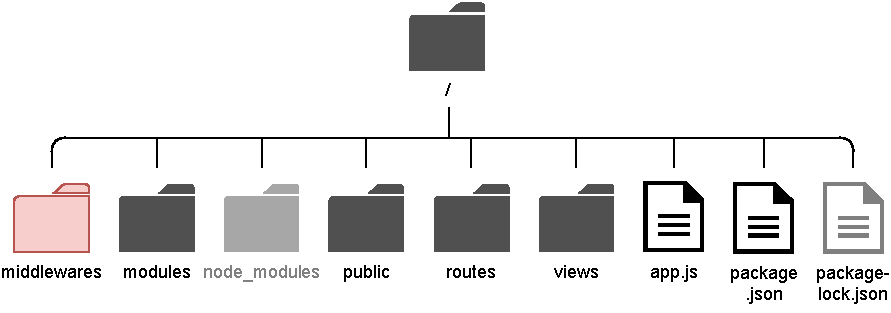
\includegraphics[width=0.75\textwidth]{includes/figures/bonus_nodejs_middlewares.pdf}
    \end{center}
\end{bonus}

\begin{defi}{Template Engine}
    Wenn man Webseiten dynamisch aufbauen möchte, ist es sinnvoll, Darstellung und Inhalt sauber zu trennen.
    Eine erste Idee ist, dass man leere \texttt{html} Seiten schreibt und in der Route füllt.

    Im weiteren nutzen wir das Modul \emph{mustache-express}
\end{defi}

\begin{example}{views (Node.js)}
    \texttt{views/pokemon.html}:
    \begin{lstlisting}[language=HTML5]
        <!DOCTYPE html>
        <html>
        <head> <title>Pokemon</title> </head>

        <body>
            <table>
                <tr> <th>ID</th> <th>Name</th> </tr>
                <tr>
                    <td>^{{id}}^</td>
                    <td>^{{name}}^</td>
                </tr>
            </table>
        </body>
        </html>
    \end{lstlisting}

    \texttt{routes/pokemon.js}:
    \begin{lstlisting}[language=JavaScript]
        const Pokemon = require('./../modules/pokemon.js')
        const express = require('express')
        
        module.exports = express.Router()
            .get('/', (req, res) => {
                const pokemon = Pokemon.get_rand()

                // render mit json Objekt, key -> Platzhalter
                res.render('pokemon.html', {
                    ^'id'^: pokemon.id,
                    ^'name'^: pokemon.name 
                })
            })
    \end{lstlisting}

    \texttt{app.js}:
    \begin{lstlisting}[language=JavaScript]
        const express = require('express')
        const mustache = require('mustache-express')

        const app = express()
        const port = 3000

        /* middlewares */
        ^app.engine('html', mustache)^           // default engine, die von res.render() genutzt wird
        ^app.set('views', __dirname + '/views')^ // Ordner, in dem die engine nach html Dateien sucht

        /* routes */
        app.use('/pokemon', require('routes/pokemon.js'))
        
        app.listen(port)
    \end{lstlisting}
\end{example}